


\tikzset{every picture/.style={line width=0.75pt}} %set default line width to 0.75pt        

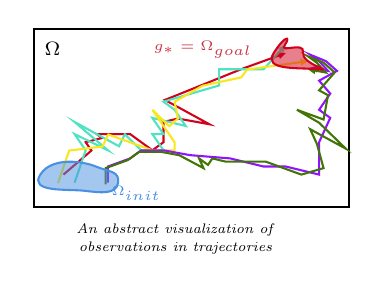
\begin{tikzpicture}[x=0.75pt,y=0.75pt,yscale=-1,xscale=1]
%uncomment if require: \path (0,1974); %set diagram left start at 0, and has height of 1974

%Shape: Rectangle [id:dp21508130618742183] 
\draw  [fill={rgb, 255:red, 255; green, 255; blue, 255 }  ,fill opacity=1 ] (27.9,1694.11) -- (180,1694.11) -- (180,1780) -- (27.9,1780) -- cycle ;
%Straight Lines [id:da4715774117452397] 
\draw [color={rgb, 255:red, 208; green, 2; blue, 27 }  ,draw opacity=1 ]   (146.57,1706.84) -- (128.18,1713.49) -- (91.16,1728.41) -- (112.58,1740.12) -- (97.43,1737.36) -- (90.48,1739.01) -- (90.48,1748.77) -- (85.95,1752.07) -- (85.12,1752.67) -- (82.55,1750.8) -- (74.41,1744.86) -- (58.34,1744.86) -- (60.9,1746.73) -- (52.99,1748.77) -- (55.75,1752.79) -- (42.28,1764.38) ;
\draw [shift={(149.39,1705.82)}, rotate = 160.12] [fill={rgb, 255:red, 208; green, 2; blue, 27 }  ,fill opacity=1 ][line width=0.08]  [draw opacity=0] (3.57,-1.72) -- (0,0) -- (3.57,1.72) -- cycle    ;
%Straight Lines [id:da12621479480258224] 
\draw [color={rgb, 255:red, 80; green, 227; blue, 194 }  ,draw opacity=1 ]   (147.37,1704.13) -- (138.68,1713.63) -- (117.26,1713.63) -- (117.26,1721.44) -- (90.48,1729.25) -- (95.83,1733.15) -- (101.19,1740.96) -- (85.12,1737.06) -- (90.48,1744.86) -- (85.12,1744.86) -- (90.48,1752.67) -- (79.77,1752.67) -- (71.84,1744.94) -- (69.05,1750.72) -- (47.63,1739.01) -- (63.7,1752.67) -- (47.63,1744.86) -- (52.99,1752.67) -- (47.63,1768.29) ;
\draw [shift={(149.39,1701.92)}, rotate = 132.45] [fill={rgb, 255:red, 80; green, 227; blue, 194 }  ,fill opacity=1 ][line width=0.08]  [draw opacity=0] (3.57,-1.72) -- (0,0) -- (3.57,1.72) -- cycle    ;
%Straight Lines [id:da7064890769152855] 
\draw [color={rgb, 255:red, 248; green, 231; blue, 28 }  ,draw opacity=1 ]   (157.13,1710.14) -- (130.73,1713.75) -- (127.97,1717.54) -- (109.3,1721.56) -- (95.83,1729.25) -- (97.43,1737.36) -- (93.24,1741.08) -- (85.12,1733.15) -- (95.83,1748.77) -- (95.83,1752.67) -- (85.12,1752.67) -- (63.89,1745.06) -- (61.1,1750.84) -- (45.04,1752.79) -- (39.68,1768.41) ;
\draw [shift={(160.1,1709.73)}, rotate = 172.2] [fill={rgb, 255:red, 248; green, 231; blue, 28 }  ,fill opacity=1 ][line width=0.08]  [draw opacity=0] (3.57,-1.72) -- (0,0) -- (3.57,1.72) -- cycle    ;
%Straight Lines [id:da7638374972620724] 
\draw [color={rgb, 255:red, 144; green, 19; blue, 254 }  ,draw opacity=1 ]   (164.12,1713.39) -- (169.74,1714.41) -- (165.46,1709.73) -- (161.17,1706.61) -- (168.76,1709.73) -- (174.03,1714.41) -- (165.46,1719.1) -- (170.81,1725.34) -- (165.46,1733.15) -- (170.81,1737.06) -- (165.46,1748.77) -- (165.46,1764.38) -- (149.39,1760.48) -- (138.68,1760.48) -- (132.88,1759.07) -- (129.82,1758.33) -- (125.47,1757.27) -- (122.61,1756.58) -- (111.86,1755.71) -- (103.33,1755.01) -- (99.13,1754.25) -- (90.48,1752.67) -- (79.77,1752.67) -- (74.41,1756.58) -- (63.7,1760.48) -- (63.7,1768.29) ;
\draw [shift={(161.17,1712.85)}, rotate = 10.33] [fill={rgb, 255:red, 144; green, 19; blue, 254 }  ,fill opacity=1 ][line width=0.08]  [draw opacity=0] (3.57,-1.72) -- (0,0) -- (3.57,1.72) -- cycle    ;
%Straight Lines [id:da2586635599751653] 
\draw [color={rgb, 255:red, 65; green, 117; blue, 5 }  ,draw opacity=1 ]   (163.05,1714.17) -- (168.67,1715.19) -- (164.39,1710.51) -- (160.1,1707.39) -- (167.69,1710.51) -- (172.95,1715.19) -- (165.46,1723.78) -- (169.74,1726.13) -- (167.6,1737.84) -- (154.75,1733.15) -- (165.46,1739.4) -- (178.31,1751.89) -- (161.17,1742.52) -- (164.39,1749.55) -- (167.6,1761.26) -- (156.89,1764.38) -- (139.75,1758.14) -- (126.9,1758.14) -- (120.47,1758.14) -- (114.04,1756.58) -- (111.9,1759.7) -- (107.62,1756.58) -- (109.76,1761.26) -- (98.06,1755.03) -- (89.41,1753.45) -- (78.69,1753.45) -- (73.34,1757.36) -- (62.63,1761.26) -- (62.63,1769.07) ;
\draw [shift={(160.1,1713.63)}, rotate = 10.33] [fill={rgb, 255:red, 65; green, 117; blue, 5 }  ,fill opacity=1 ][line width=0.08]  [draw opacity=0] (3.57,-1.72) -- (0,0) -- (3.57,1.72) -- cycle    ;
%Shape: Polygon Curved [id:ds11407168049221061] 
\draw  [color={rgb, 255:red, 74; green, 144; blue, 226 }  ,draw opacity=1 ][fill={rgb, 255:red, 74; green, 144; blue, 226 }  ,fill opacity=0.5 ] (31.11,1764.38) .. controls (34.28,1759.39) and (40.53,1757.99) .. (46.46,1758.18) .. controls (50.95,1758.33) and (55.26,1759.39) .. (57.89,1760.48) .. controls (64,1763.02) and (69.46,1762.63) .. (68.6,1768.29) .. controls (67.74,1773.95) and (60.78,1773.17) .. (52.53,1772.19) .. controls (44.29,1771.22) and (25.54,1773.17) .. (31.11,1764.38) -- cycle ;
%Shape: Polygon Curved [id:ds9280877944894264] 
\draw  [color={rgb, 255:red, 208; green, 2; blue, 27 }  ,draw opacity=1 ][fill={rgb, 255:red, 208; green, 2; blue, 27 }  ,fill opacity=0.5 ] (143.58,1705.82) .. controls (149.15,1697.04) and (151.91,1697.59) .. (148.94,1701.92) .. controls (145.97,1706.25) and (158.58,1699.87) .. (157.72,1705.53) .. controls (156.86,1711.19) and (173.25,1714.61) .. (165,1713.63) .. controls (156.76,1712.66) and (138.01,1714.61) .. (143.58,1705.82) -- cycle ;


% Text Node
\draw (109.47,1704.35) node  [font=\tiny,color={rgb, 255:red, 202; green, 52; blue, 69 }  ,opacity=1 ] [align=left] {$\displaystyle g_{*} =\Omega _{goal}$};
% Text Node
\draw (77.33,1773.35) node  [font=\tiny,color={rgb, 255:red, 74; green, 144; blue, 226 }  ,opacity=1 ] [align=left] {$\displaystyle \Omega _{init}$};
% Text Node
\draw (37,1704) node  [font=\scriptsize] [align=left] {$\displaystyle \Omega $};
% Text Node
\draw (96.51,1791) node   [align=left] {{\tiny \textit{An abstract visualization of}}};
\draw (96.51,1800) node   [align=left] {{\tiny \textit{observations in trajectories}}};

\end{tikzpicture}